%%%%%%%%%%%%%%%%%%%%%%%%%%%%%%%%%%%%%%%%%
% Jacobs Landscape Poster
% LaTeX Template
% Version 1.1 (14/06/14)
%
% Created by:
% Computational Physics and Biophysics Group, Jacobs University
% https://teamwork.jacobs-university.de:8443/confluence/display/CoPandBiG/LaTeX+Poster
% 
% Further modified by:
% Nathaniel Johnston (nathaniel@njohnston.ca)
%
% This template has been downloaded from:
% http://www.LaTeXTemplates.com
%
% License:
% CC BY-NC-SA 3.0 (http://creativecommons.org/licenses/by-nc-sa/3.0/)
%
%%%%%%%%%%%%%%%%%%%%%%%%%%%%%%%%%%%%%%%%%

%----------------------------------------------------------------------------------------
%	PACKAGES AND OTHER DOCUMENT CONFIGURATIONS
%----------------------------------------------------------------------------------------

\documentclass[final]{beamer}
\documentclass[conference]{IEEEtran}

% Make latex understand and use the typographic
% rules of the language used in the document.
\usepackage[english]{babel}
\usepackage[utf8]{inputenc}
% Choose the font encoding
\usepackage[T1]{fontenc}

% Use colour in tables
\usepackage[table]{xcolor}
\usepackage{array}
\usepackage{multirow}

% load a colour package
\usepackage{xcolor}
\definecolor{aaublue}{RGB}{33,26,82}% dark blue

% The standard graphics inclusion package
\definecolor{white}{RGB}{255,255,255} % define color white
\usepackage{graphicx}

% Set up how figure and table captions are displayed
\usepackage{caption}
\captionsetup{
  font=footnotesize,% set font size to footnotesize
  labelfont=bf % bold label (e.g., Figure 3.2) font
}

% Enable row combination in tables
\usepackage{multirow}

% Make space between table lines and text
\renewcommand{\arraystretch}{1.5}

% Make the standard latex tables look so much better
\usepackage{array,booktabs}



%%%%%%%%%%%%%%%%%%%%%%%%%%%%%%%%%%%%%%%%%%%%%%%%
% Mathematics
%%%%%%%%%%%%%%%%%%%%%%%%%%%%%%%%%%%%%%%%%%%%%%%%
% Defines new environments such as equation,
% align and split 
\usepackage{amsmath}
\usepackage{relsize}
% Adds new math symbols
\usepackage{amssymb}
% Use theorems in your document
% The ntheorem package is also used for the example environment
% When using thmmarks, amsmath must be an option as well. Otherwise \eqref doesn't work anymore.
\usepackage[framed,amsmath,thmmarks]{ntheorem}
\usepackage{cancel}

%%%%%%%%%%%%%%%%%%%%%%%%%%%%%%%%%%%%%%%%%%%%%%%%
% Page Layout
%%%%%%%%%%%%%%%%%%%%%%%%%%%%%%%%%%%%%%%%%%%%%%%%


%%%%%%%%%%%%%%%%%%%%%%%%%%%%%%%%%%%%%%%%%%%%%%%%
% Bibliography
%%%%%%%%%%%%%%%%%%%%%%%%%%%%%%%%%%%%%%%%%%%%%%%%
%%setting references (using numbers) and supporting i.a. Chicargo-style:
\usepackage{etex}
\usepackage{etoolbox}
\usepackage{keyval}
\usepackage{ifthen}
\usepackage{url}
\usepackage{csquotes}
\usepackage[backend=biber, url=true, doi=true, citestyle=ieee, bibstyle=ieee, sorting=none]{biblatex}
\addbibresource{setup/bibliography.bib}

%%%%%%%%%%%%%%%%%%%%%%%%%%%%%%%%%%%%%%%%%%%%%%%%
% Misc
%%%%%%%%%%%%%%%%%%%%%%%%%%%%%%%%%%%%%%%%%%%%%%%%

%%% Enables the use FiXme refferences. Syntax: \fxnote{...} %%%
\usepackage[footnote, draft, english, silent, nomargin]{fixme}
%With "final" instead of "draft" an error will ocure for every FiXme under compilation.

%%% allows use of lorem ipsum (generate i.e. pagagraph 1 to 5 with \lipsum[1-5]) %%%
\usepackage{lipsum}

%%% Enables figures with text wrapped tightly around it %%%
\usepackage{wrapfig}

\usepackage{float}
\usepackage{caption}
\usepackage{subcaption}
\usepackage{siunitx}
\sisetup{decimalsymbol=comma}
\sisetup{detect-weight}

\usepackage{enumitem}
%\usepackage[citestyle=authoryear,natbib=true]{biblatex}

% Figures - TIKZ
\usepackage{tikz}
\usetikzlibrary{shapes,arrows}
\usepackage[americanresistors,americaninductors,americancurrents, americanvoltages]{circuitikz}

% Wall of text logo
\newcommand{\walloftextalert}[0]{\includegraphics[width=\textwidth]{walloftext.png}}

\usepackage{pdfpages}
\usepackage{lastpage}
\usepackage{epstopdf}

\setlength{\headheight}{21pt}

\hfuzz=\maxdimen
\tolerance = 10000
\hbadness  = 10000

\usepackage{siunitx}
\graphicspath{{./figures/}}% package inclusion and set up of the document

%%%%%%%%%%%%%%%%%%%%%%%%%%%%%%%%%%%%%%%%%%%%%%%%%%%%%
%             UNITS, EQUATIONS AND TEXT             %
%%%%%%%%%%%%%%%%%%%%%%%%%%%%%%%%%%%%%%%%%%%%%%%%%%%%%
%Units:
\newcommand{\unit}[1]{&& \left[\si{#1}\right]} %\newcommand{\unit}[1]{[\si{#1}]}             <<| Use these if you want uations to be
\newcommand{\unitWh}[1]{[\si{#1}]}             %\newcommand{\eq}[2]{&&\si{#1} &= \si{#2}&&}  <<| centered.. .. will appear scrambled
\newcommand{\numUnit}[1]{\ \si{#1}&}           %                                               | from one equation to the next though..
%Equation:                                     %                                               | and does not work with long equations.. :/
\newcommand{\eq}[2]{\si{#1} &= \si{#2}}
\newcommand{\arw}{&& &\Updownarrow&&}
\newcommand{\eqOne}[2]{\si{#1} &= \si{#2} &\nonumber\\}
\newcommand{\eqTwo}[1]{&\ \ \ \ \si{#1}& \nonumber\\}
\newcommand{\eqThree}[1]{&\ \ \ \ \si{#1}&}
%Text:
\newcommand{\tx}[1]{\text{#1}}
%Vectors
\renewcommand{\vec}[1]{\boldsymbol{\mathbf{#1}}}
%Vertical line in equations ie. |_x=y (whereTwo stacks two equalities at the line)
\newcommand{\lineWhere}[1]{ \left.\rule{0cm}{.5cm}\right\vert\rule{0cm}{.4cm}_{\substack{\rule{0cm}{.15cm}\\ \si{#1} }} }
\newcommand{\lineWhereTwo}[2]{ \left.\rule{0cm}{.67cm}\right\vert\rule{0cm}{.5cm}_{\substack{\si{#1} \rule{0cm}{.19cm}\\\vspace{-.1cm}\\ \si{#2}}} }

%%%%%%%%%%%%%%%%%%%%%%%%%%%%%%%%%%%%%%%%%%%%%%%%%%%%%
%                 TIKZ SETTINGS                     %
%%%%%%%%%%%%%%%%%%%%%%%%%%%%%%%%%%%%%%%%%%%%%%%%%%%%%
%\usetikzlibrary{arrows.meta}
\tikzset{
  block/.style    = {draw, thick, rectangle,
                     minimum height = 2.1em,
                     minimum width = 1.7em},
  sum/.style      = {draw, circle, inner sep=1.5pt},
}

%%%%%%%%%%%%%%%%%%%%%%%%%%%%%%%%%%%%%%%%%%%%%%%%%%%%%
%               WHERE, AFTER MATH                   %
%%%%%%%%%%%%%%%%%%%%%%%%%%%%%%%%%%%%%%%%%%%%%%%%%%%%%
\usepackage{xifthen}

\newenvironment{where}{\par\vspace{-4mm}\noindent\ignorespaces Where:\\}{\\}
\newcommand{\va}[3]
{
  \begin{tabular}{p{10pt} p{145pt} l}
    { $#1$ } & { #2 } & \ifthenelse{\isempty{ #3 }}  {}  {[{\si{#3}}]} \\
  \end{tabular}\\
}% my new macros

\usepackage[scale=1.24]{beamerposter} % Use the beamerposter package for laying out the poster

\usetheme{confposter} % Use the confposter theme supplied with this template

%\setbeamercolor{block title}{fg=black,bg=white} % Colors of the block titles
%\setbeamercolor{block body}{fg=black,bg=white} % Colors of the body of blocks
%\setbeamercolor{block alerted title}{fg=white,bg=dblue!70} % Colors of the highlighted block titles
\setbeamercolor{block alerted body}{fg=black,bg=white} % Colors of the body of highlighted blocks
% Many more colors are available for use in beamerthemeconfposter.sty

%-----------------------------------------------------------
% Define the column widths and overall poster size
% To set effective sepwid, onecolwid and twocolwid values, first choose how many columns you want and how much separation you want between columns
% In this template, the separation width chosen is 0.024 of the paper width and a 4-column layout
% onecolwid should therefore be (1-(# of columns+1)*sepwid)/# of columns e.g. (1-(4+1)*0.024)/4 = 0.22
% Set twocolwid to be (2*onecolwid)+sepwid = 0.464
% Set threecolwid to be (3*onecolwid)+2*sepwid = 0.708

\newlength{\sepwid}
\newlength{\onecolwid}
\newlength{\twocolwid}
\newlength{\threecolwid}
\setlength{\paperwidth}{48in} % A0 width: 46.8in
\setlength{\paperheight}{36in} % A0 height: 33.1in
\setlength{\sepwid}{0.024\paperwidth} % Separation width (white space) between columns
\setlength{\onecolwid}{0.22\paperwidth} % Width of one column
\setlength{\twocolwid}{0.464\paperwidth} % Width of two columns
\setlength{\threecolwid}{0.708\paperwidth} % Width of three columns
\setlength{\topmargin}{-0.5in} % Reduce the top margin size
%-----------------------------------------------------------

\usepackage{graphicx}  % Required for including images

\usepackage{booktabs} % Top and bottom rules for tables


%----------------------------------------------------------------------------------------
%	TITLE SECTION 
%----------------------------------------------------------------------------------------

\title{Attitude and Position Control of a Quadcopter in a Networked \\	Distributed System} % Poster title

\author{Alejandro Alonso García, Amalie V. Petersen, Andrea Victoria Tram Løvemærke,\\ Niels Skov Vestergaard, Noelia Villarmarzo Arruñada} % Author(s)

\institute{	Email: [aalons16] [apet13] [alavem13] [nveste12] [nvilla16] @student.aau.dk} % Institution(s)

\addtobeamertemplate{headline}{} 
{
	\begin{tikzpicture}[remember picture,overlay] 
	\node [shift={(-15 cm,-11cm)}] at (current page.north east) {\includegraphics[height=9cm]{figures/aau_logo_cropped}}; 
	\end{tikzpicture} 
}
%----------------------------------------------------------------------------------------

\begin{document}

\addtobeamertemplate{block end}{}{\vspace*{2ex}} % White space under blocks
\addtobeamertemplate{block alerted end}{}{\vspace*{2ex}} % White space under highlighted (alert) blocks

\setlength{\belowcaptionskip}{2ex} % White space under figures
\setlength\belowdisplayshortskip{2ex} % White space under equations

\begin{frame}[t] % The whole poster is enclosed in one beamer frame

\begin{columns}[t] % The whole poster consists of three major columns, the second of which is split into two columns twice - the [t] option aligns each column's content to the top

\begin{column}{\sepwid}\end{column} % Empty spacer column

\begin{column}{\onecolwid} % The first column

%----------------------------------------------------------------------------------------
%	INTRODUCTION
%----------------------------------------------------------------------------------------

\begin{block}{Introduction}
%In the last years, the interest for quadcopters has increased due to the great possibilities they offer. Among these, the most well-known ones are surveillance, inspection of big structures and search and rescue missions in difficult environments.
A design that is able to make the quadcopter hover and move to a desired position is designed. The system’s coupled behavior and instability raises a challenging control task.

This task is solved by implementing a linear control design. The system is split into an attitude and translational model. These are controlled individually by state space and classical controllers respectively. The prototype gets its attitude and position from a motion tracking system based on infrared cameras, keeping the control in a micro processor on the quadcopter. This layout constitutes a distributed system, where network issues, such as delays and packet losses, are taken into account.
\end{block}

%----------------------------------------------------------------------------------------
%	METHODS
%----------------------------------------------------------------------------------------

\begin{block}{Methods}


\begin{figure}
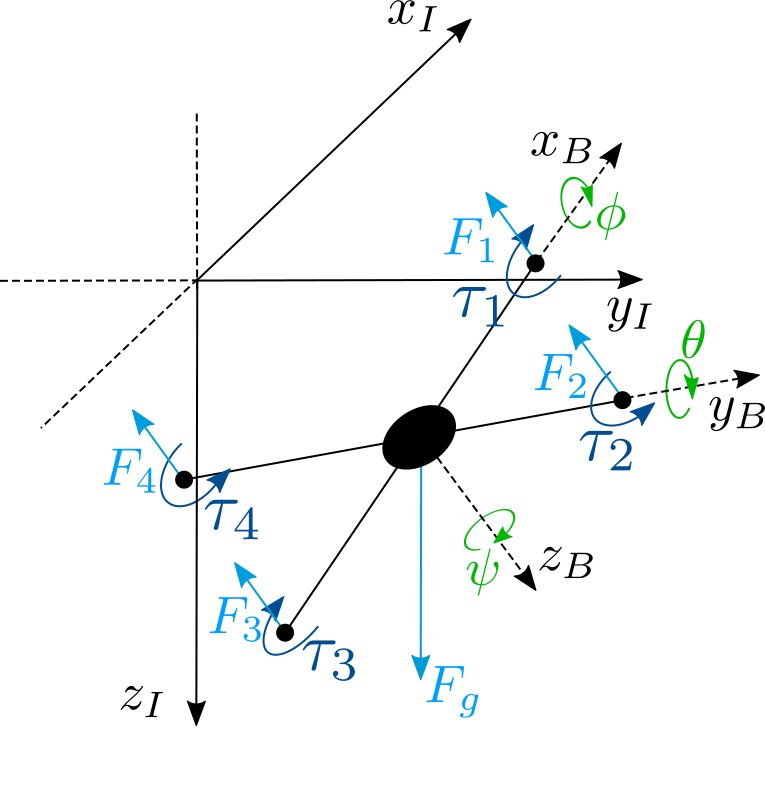
\includegraphics[width=0.8\linewidth]{figures/droneDiagram.pdf}
\caption{Free body diagram of the quadcopter along with the inertial and body coordinate systems.}
\end{figure}
The system is modeled by using two coordinate frames. The inertial frame is utilized to describe the translational movement while the body frame is attached to the quadcopter and used to characterize its attitude behavior.
This statement requires citation \cite{Smith:2012qr}.

\end{block}

%------------------------------------------------

%\begin{figure}
%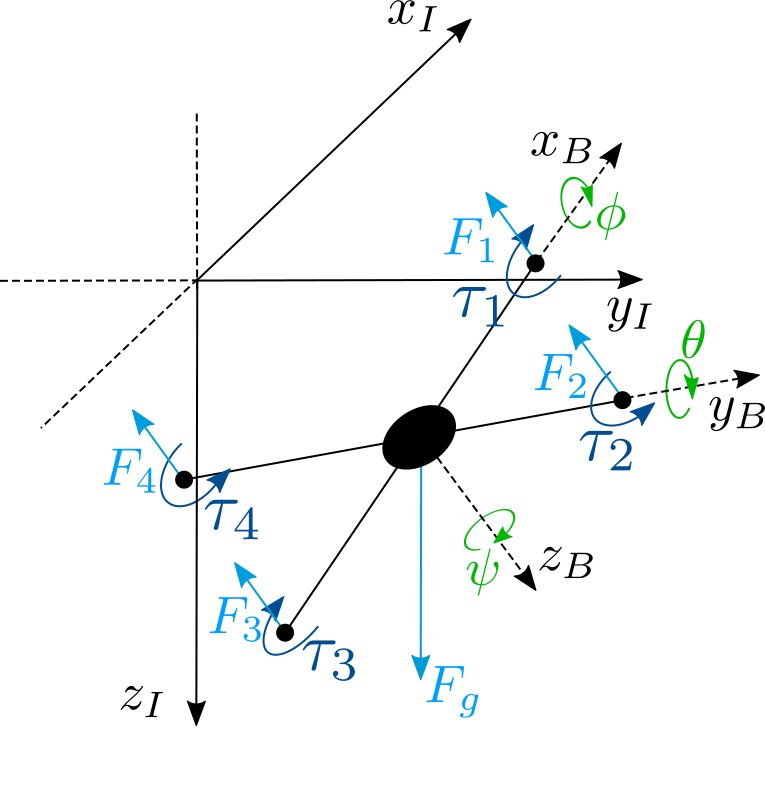
\includegraphics[width=0.8\linewidth]{figures/droneDiagram.pdf}
%\caption{Figure caption}
%\end{figure}

%----------------------------------------------------------------------------------------

\end{column} % End of the first column

\begin{column}{\sepwid}\end{column} % Empty spacer column

\begin{column}{\twocolwid} % Begin a column which is two columns wide (column 2)

\begin{columns}[t,totalwidth=\twocolwid] % Split up the two columns wide column

\begin{column}{\onecolwid}\vspace{-.6in} % The first column within column 2 (column 2.1)

%----------------------------------------------------------------------------------------
%	RESULTS
%----------------------------------------------------------------------------------------
\begin{block}{Method}
The attitude model equations for rotational movement is as follows 
\begin{flalign}
	J_x\ddot{\phi}&=k_{\mathrm{th}} (\omega^2_4-\omega^2_2)  L \label{eq:AngleEqVelocities1}\\
	J_y\ddot{\theta}&=k_{\mathrm{th}} (\omega^2_1-\omega^2_3)  L \label{eq:AngleEqVelocities2} \\
	J_z\ddot{\psi}&=k_{\mathrm{d}} (\omega^2_1-\omega^2_2+\omega^2_3-\omega^2_4)\label{eq:AngleEqVelocities3}
\end{flalign}
The response of the system along the inertial x, y and z axes are derived from Newton's Second Law of Motion, as follows
\begin{flalign}
     m\ddot{x}_{\mathrm{I}} = &-k_{\mathrm{th}} ({\omega_1}^2+{\omega_2}^2+{\omega_3}^2+{\omega_4}^2) \label{eq:AccelerationEqInertial1}\\
     & \ \times (\cos\phi \sin\theta \cos\psi + \sin\phi\sin\psi)   \nonumber\\
     m \ddot{y}_{\mathrm{I}} = &-k_{\mathrm{th}}({\omega_1}^2+{\omega_2}^2+{\omega_3}^2+{\omega_4}^2) \label{eq:AccelerationEqInertial2}\\
     & \ \times(\cos\phi \sin\theta \sin\psi - \sin\phi \cos\psi)  \nonumber\\
     m\ddot{z}_{\mathrm{I}} = &F_g-k_{\mathrm{th}}\ ({\omega_1}^2+{\omega_2}^2+{\omega_3}^2+{\omega_4}^2) \label{eq:AccelerationEqInertial3}\\
     & \ \times \cos\phi\cos\theta  \nonumber
\end{flalign}

%
%\begin{figure}
%\includegraphics[width=0.8\linewidth]{figures/AttitudeControl.pdf}
%\caption{Figure caption}
%\end{figure}
%The materials were prepared according to the steps outlined below:
%\begin{enumerate}
%\item Template
%\item Template
%\end{enumerate}

\end{block}

%----------------------------------------------------------------------------------------

\end{column} % End of column 2.1

\begin{column}{\onecolwid}\vspace{-.6in} % The second column within column 2 (column 2.2)

%----------------------------------------------------------------------------------------
%	RESULTS
%----------------------------------------------------------------------------------------

\begin{block}{Results}
\begin{figure}
\includegraphics[width=0.8\linewidth]{figures/AttitudeControl.pdf}
\caption{Figure caption}
\end{figure}
\end{block}

%----------------------------------------------------------------------------------------

\end{column} % End of column 2.2

\end{columns} % End of the split of column 2 - any content after this will now take up 2 columns width

%----------------------------------------------------------------------------------------
%	IMPORTANT RESULT
%----------------------------------------------------------------------------------------

\begin{alertblock}{Important Result}

This is for bringing the final controller graph with some text saying, it hopefully works well.
\begin{figure}
\includegraphics[width=0.5\linewidth]{figures/PositionControl.pdf}
\caption{Figure caption}
\end{figure}


\end{alertblock} 

%----------------------------------------------------------------------------------------

\begin{columns}[t,totalwidth=\twocolwid] % Split up the two columns wide column again

\begin{column}{\onecolwid} % The first column within column 2 (column 2.1)

%----------------------------------------------------------------------------------------
%	MATHEMATICAL SECTION
%----------------------------------------------------------------------------------------

%\begin{block}{Mathematical Section}

%MATH
  
%\begin{equation}
%E = mc^{2}
%\label{eqn:Einstein}
%\end{equation}



%\begin{equation}
%\cos^3 \theta =\frac{1}{4}\cos\theta+\frac{3}{4}\cos 3\theta
%\label{eq:refname}
%\end{equation}

%
%\begin{equation}
%\kappa =\frac{\xi}{E_{\mathrm{max}}} %\mathbb{ZNR}
%\end{equation}
%
%\end{block}

%----------------------------------------------------------------------------------------

\end{column} % End of column 2.1

\begin{column}{\onecolwid} % The second column within column 2 (column 2.2)

%----------------------------------------------------------------------------------------
%	RESULTS
%----------------------------------------------------------------------------------------

%\begin{block}{Results}
%
%\begin{table}
%\vspace{2ex}
%\begin{tabular}{l l l}
%\toprule
%\textbf{Treatments} & \textbf{Response 1} & \textbf{Response 2}\\
%\midrule
%Treatment 1 & 0.0003262 & 0.562 \\
%Treatment 2 & 0.0015681 & 0.910 \\
%Treatment 3 & 0.0009271 & 0.296 \\
%\bottomrule
%\end{tabular}
%\caption{Table caption}
%\end{table}
%
%\end{block}

%----------------------------------------------------------------------------------------

\end{column} % End of column 2.2

\end{columns} % End of the split of column 2

\end{column} % End of the second column

\begin{column}{\sepwid}\end{column} % Empty spacer column

\begin{column}{\onecolwid} % The third column

%----------------------------------------------------------------------------------------
%	Results
%----------------------------------------------------------------------------------------

\begin{block}{ }
The attitude controller is defined by the chosen feedback and integral poles, \\$[-6.0, -6.2, -6.4, -6.6, -6.8, -7.0, -7.2, -7.4, -7.6]$, and  the observer poles, $[-20, -25, -30]$.
The translation velocity controllers for x and y are $C_{\dot{x}}(s)= -0.1$, $C_{\dot{y}}(s)= 0.1$ and the position ones are $C_x(s)= 0.5$, $C_y(s)= 0.5$. The PI-controller for the z translational velocity is $C_{\dot{z}}(s)=-201\frac{s+0.8}{s}$ and the outer loop P-controller is $C_z=0.9$.
\end{block}
%----------------------------------------------------------------------------------------
%	DISCUSSION
%----------------------------------------------------------------------------------------

\begin{block}{Discussion}
It is seen that the controllers achieve the desired reference even though the network delay and the sampling rate affect the performance. The main network effect is the designed bandwidth of the controllers. This occurs due to the limited frequency in which the sensor data is obtained from the motion tracking system through the wireless connection.
\end{block}

%----------------------------------------------------------------------------------------
%	Conclusion
%----------------------------------------------------------------------------------------

\begin{block}{Conclusion}
The control system has been split into an attitude and a translational controller. The former has been designed using a state space approach, including state feedback with integral control and a reduced order observer. The translational control system has been designed with a classical control approach and result in three cascade loops, including proportional and PI controllers.
The results obtained from the design show that both the attitude and the translational behavior of the quadcopter has been successfully controlled.
\end{block}

%----------------------------------------------------------------------------------------
%	References
%----------------------------------------------------------------------------------------

\begin{block}{References}

\small{\rmfamily{CONTROL BOOK.}} \\
%\nocite{*} % Insert publications even if they are not cited in the poster
%\small{\bibliographystyle{unsrt}
%\bibliography{sample}\vspace{0.75in}}
\printbibliography
\end{block}

%----------------------------------------------------------------------------------------
%	Acknowledgements
%----------------------------
\begin{block}{Acknowledgements}

\small{\rmfamily{Henrik Shøiler, Assosiated Proffesor, Aalborg University.\\
Christoffer Sloth, Assosiated Professor, Aalborg University.}} \\
\end{block}
%----------------------------------------------------------------------------------------
%	CONTACT INFORMATION
%----------------------------------------------------------------------------------------

%\setbeamercolor{block alerted title}{fg=black,bg=norange} % Change the alert block title colors
%\setbeamercolor{block alerted body}{fg=black,bg=white} % Change the alert block body colors
%
%\begin{alertblock}{Contact Information}
%
%\begin{itemize}
%\item Web: \href{http://www.university.edu/smithlab}{http://www.university.edu/smithlab}
%\item Email: \href{mailto:john@smith.com}{john@smith.com}
%\item Phone: +1 (000) 111 1111
%\end{itemize}
%
%\end{alertblock}
%
%\begin{center}
%\begin{tabular}{ccc}
%\includegraphics[width=0.4\linewidth]{logo.png} & \hfill & \includegraphics[width=0.4\linewidth]{logo.png}
%\end{tabular}
%\end{center}

%----------------------------------------------------------------------------------------

\end{column} % End of the third column

\end{columns} % End of all the columns in the poster
\tikz[remember picture,overlay] \node[opacity=0.7,inner sep=0pt] at (current page.center){\includegraphics[width=\paperwidth,height=\paperheight]{figures/drawing}};
\clearpage
\end{frame} % End of the enclosing frame

\end{document}
